\documentclass[aspectratio=169,11pt]{beamer}

\usetheme{default}
\setbeamertemplate{navigation symbols}{}
\setbeamertemplate{footline}[frame number]
\usepackage{amsmath,amssymb}
\usepackage{booktabs}
\usepackage{multirow}
\usepackage{tikz}
\usetikzlibrary{calc,decorations.pathreplacing}
\usepackage{nicematrix}

\newcommand{\lc}{\textsc{l}}              % left child
\newcommand{\rc}{\textsc{r}}              % right child
\newcommand{\Par}{\mathcal{P}}            % parent
\newcommand{\Ecount}{\mathcal{E}}         % number of border edges

\colorlet{nz}{blue!35}        % nonzero entry of T_k
\colorlet{hank}{orange!20}    % Hankel block
\colorlet{hit}{red!75}        % nonzero of T_k inside the Hankel block
\colorlet{inA}{orange!70}     % nodes of the set A

% The level-4 tree (post-ordered, root 15). Leaves on y=0, root on y=3.
\newcommand{\treefourcoords}{%
\foreach \k/\x in {1/0,2/1,4/2,5/3,8/4,9/5,11/6,12/7} \coordinate (t\k) at (\x,0);
\foreach \k/\x in {3/0.5,6/2.5,10/4.5,13/6.5} \coordinate (t\k) at (\x,1);
\coordinate (t7) at (1.5,2); \coordinate (t14) at (5.5,2); \coordinate (t15) at (3.5,3);}
\newcommand{\treefouredges}{1/3,2/3,4/6,5/6,3/7,6/7,8/10,9/10,11/13,12/13,10/14,13/14,7/15,14/15}
% \treefour{nodes of A}{border edges}: the level-4 tree with A filled and the border edges in red
\newcommand{\treefour}[2]{%
\begin{tikzpicture}[x=7mm,y=\treey]
\treefourcoords
\foreach \c/\p in \treefouredges \draw[thick] (t\c) -- (t\p);
\foreach \c/\p in {#2} \draw[hit,line width=2pt] (t\c) -- (t\p);
\foreach \k in {1,...,15} \fill (t\k) circle (1.6pt);
\foreach \k in {#1} \fill[inA,draw=black] (t\k) circle (2.6pt);
\foreach \k in {1,2,4,5,8,9,11,12} \node[font=\scriptsize,below=2pt] at (t\k) {$\k$};
\foreach \k in {3,7,10} \node[font=\scriptsize,above left=0pt] at (t\k) {$\k$};
\foreach \k in {6,13,14} \node[font=\scriptsize,above right=0pt] at (t\k) {$\k$};
\node[font=\scriptsize,above=2pt] at (t15) {$\mathbf{15}$};
\end{tikzpicture}}

% level order of the level-4 tree: node j has parent floor(j/2)
\newcommand{\levelfouredges}{2/1,3/1,4/2,5/2,6/3,7/3,8/4,9/4,10/5,11/5,12/6,13/6,14/7,15/7}
% \treefourlevel{nodes of A}{border edges}: as \treefour (arguments in post-order labels),
% but the nodes are labelled by their position in the level order
\newcommand{\treefourlevel}[2]{%
\begin{tikzpicture}[x=7mm,y=\treey]
\treefourcoords
\foreach \c/\p in \treefouredges \draw[thick] (t\c) -- (t\p);
\foreach \c/\p in {#2} \draw[hit,line width=2pt] (t\c) -- (t\p);
\foreach \k in {1,...,15} \fill (t\k) circle (1.6pt);
\foreach \k in {#1} \fill[inA,draw=black] (t\k) circle (2.6pt);
\foreach \k/\l in {1/8,2/9,4/10,5/11,8/12,9/13,11/14,12/15} \node[font=\scriptsize,below=2pt] at (t\k) {$\l$};
\foreach \k/\l in {3/4,7/2,10/6} \node[font=\scriptsize,above left=0pt] at (t\k) {$\l$};
\foreach \k/\l in {6/5,13/7,14/3} \node[font=\scriptsize,above right=0pt] at (t\k) {$\l$};
\node[font=\scriptsize,above=2pt] at (t15) {$\mathbf{1}$};
\end{tikzpicture}}
% \clusterpanel{S nodes}{R nodes}{single nodes}{edges inside S clusters}{edges inside R clusters}:
% the level-4 tree with the clusters of one depth of the subtree-aligned cluster tree. Edges between
% two clusters (already cut) are red and dashed.
\colorlet{clS}{blue!55}
\colorlet{clR}{orange!85}
\colorlet{clV}{gray!55}
\newcommand{\clusterpanel}[5]{%
\begin{tikzpicture}[x=4.4mm,y=6mm]
\treefourcoords
\foreach \c/\p in \treefouredges \draw[hit,dashed,line width=0.8pt] (t\c) -- (t\p);
\foreach \c/\p in {#4} \draw[clS,line width=2.4pt] (t\c) -- (t\p);
\foreach \c/\p in {#5} \draw[clR,line width=2.4pt] (t\c) -- (t\p);
\foreach \k in {#1} \fill[clS,draw=black] (t\k) circle (2.4pt);
\foreach \k in {#2} \fill[clR,draw=black] (t\k) circle (2.4pt);
\foreach \k in {#3} \fill[clV,draw=black] (t\k) circle (2.4pt);
\foreach \k in {1,2,4,5,8,9,11,12} \node[font=\tiny,below=1.5pt] at (t\k) {$\k$};
\foreach \k in {3,7,10} \node[font=\tiny,above left=-0.5pt] at (t\k) {$\k$};
\foreach \k in {6,13,14} \node[font=\tiny,above right=-0.5pt] at (t\k) {$\k$};
\node[font=\tiny,above=1.5pt] at (t15) {$15$};
\end{tikzpicture}}
\newcommand{\treey}{8mm}     % level spacing of \treefour
\newcommand{\spyunit}{3.3mm} % cell size of \spyfour
% \spyfour{shading}{red cells i/j}: nonzero pattern of T_4. The shading argument is drawn
% first (cell (i,j) is the square (j-1,i-1)--(j,i)); the listed cells are drawn in red.
\newcommand{\spyfour}[2]{\spyfourwith{\treefouredges}{#1}{#2}}
% \spyfourwith{edge list}{shading}{red cells}: the same for another labelling of the nodes
\newcommand{\spyfourwith}[3]{\spyfourcore{#1}{#2}{#3}{}}
% \spyfourclusters{intervals a/b}: T_4 in post-order with the clusters a..b of an HSS cluster tree boxed
\newcommand{\spyfourclusters}[1]{\spyfourcore{\treefouredges}{}{}{%
  \foreach \a/\b in {#1} \draw[black,line width=0.9pt] (\a-1,\a-1) rectangle (\b,\b);}}
% \spyfourcore{edge list}{shading}{red cells}{overlay drawn last}
\newcommand{\spyfourcore}[4]{%
\begin{tikzpicture}[x=\spyunit,y=-\spyunit]
#2
\foreach \i in {1,...,15} \fill[nz] (\i-1,\i-1) rectangle (\i,\i);
\foreach \c/\p in #1 {
  \fill[nz] (\c-1,\p-1) rectangle (\c,\p);
  \fill[nz] (\p-1,\c-1) rectangle (\p,\c);}
\foreach \i/\j in {#3} \fill[hit] (\j-1,\i-1) rectangle (\j,\i);
\draw[gray!50,line width=0.2pt] (0,0) grid (15,15);
\draw[line width=0.8pt] (0,0) rectangle (15,15);
#4
\foreach \k in {1,3,7,11,15} {
  \node[font=\tiny] at (\k-0.5,-0.6) {$\k$};
  \node[font=\tiny] at (-0.7,\k-0.5) {$\k$};}
\end{tikzpicture}}

% a divider slide at the start of every section
\AtBeginSection[]{%
\begin{frame}[plain]
\vfill
\centering
{\usebeamercolor[fg]{title}\Large\insertsectionhead\par}
\vfill
\end{frame}}

\title{Can the TQS format give asymptotically\\ more compression than pure HSS?}
\subtitle{The example of Section 3.5 of the TQS paper}
\date{}

\begin{document}

\begin{frame}
\titlepage
\end{frame}

\begin{frame}[plain]
\vfill
\centering
\large If you are short on time, see slides \hyperlink{sl:thm2}{\pageref{sl:thm2}},
\hyperlink{sl:cor3}{\pageref{sl:cor3}} and \hyperlink{sl:answer}{\pageref{sl:answer}}.
\vfill
\end{frame}

\section{Recap: the example of the original paper}

\begin{frame}{Notation}
\begin{columns}[T]
\begin{column}{0.49\textwidth}
\scriptsize
\renewcommand{\arraystretch}{1.1}
\setlength{\tabcolsep}{4pt}
\begin{tabular}{@{}ll@{}}
\multicolumn{2}{@{}l}{\textbf{Tree}} \\
$\mathbb{G}_k=(\mathbb{V},\mathbb{E})$ & regular binary tree with $k$ levels \\
$K$ & number of nodes, $K=2^k-1$ \\
labels & post-order: children before parent, \\ & left subtree before right subtree \\
root & node $K$ (last in post-order) \\
$\Par(i)$ & parent of node $i\neq K$ \\
$\lc(i)$, $\rc(i)$ & left / right child of a non-leaf $i$ \\
$\mathcal{C}(i)$ & set of children of $i$ \\
$(i,j)\in\mathbb{E}$ & edge between nodes $i$ and $j$ \\
$\mathcal{S}(v)$ & nodes of the subtree rooted at $v$ \\[3pt]
\multicolumn{2}{@{}l}{\textbf{Sparse matrix}} \\
$\mathrm{T}_k$ & $K\times K$ matrix with adjacency graph $\mathbb{G}_k$ \\
$d^i$ & diagonal entry $\mathrm{T}_k(i,i)$ \\
$b^i_{\Par(i)}$ & entry $\mathrm{T}_k(\Par(i),i)$: child $\to$ parent \\
$p^{\Par(i)}_i$ & entry $\mathrm{T}_k(i,\Par(i))$: parent $\to$ child
\end{tabular}
\end{column}
\begin{column}{0.49\textwidth}
\scriptsize
\renewcommand{\arraystretch}{1.1}
\setlength{\tabcolsep}{4pt}
\begin{tabular}{@{}ll@{}}
\multicolumn{2}{@{}l}{\textbf{Rank structure}} \\
$\mathrm{T}(I,J)$ & rows $I$, columns $J$ of $\mathrm{T}$ \\
$\bar{A}$ & complement $\mathbb{V}\setminus A$ of $A\subset\mathbb{V}$ \\
Hankel block & $\mathrm{T}(\bar{A},A)$, induced by $A$ \\
border edge & $(i,j)\in\mathbb{E}$ with $i\in A$, $j\in\bar{A}$ \\
$\Ecount(A)$ & number of border edges of $A$ \\[3pt]
\multicolumn{2}{@{}l}{\textbf{TQS representation}} \\
$\rho_e$ & state dimension on edge $e$ \\ $\{\rho_e\}_{e\in\mathbb{E}}$ & rank profile \\
$\mathrm{Inp}^k_j$ & input $x_k\to$ state on edge $(k,j)$ \\
$\mathrm{Trans}^k_{i,j}$ & state on $(j,k)\to$ state on $(k,i)$ \\
$\mathrm{Out}^k_i$ & state on $(i,k)\to$ output $b_k$ \\
$\mathrm{D}^k$ & input $x_k\to$ output $b_k$ \\
$\mathrm{S}^k$ & spinner: all generators of node $k$ \\
\multicolumn{2}{@{}l}{\scriptsize With a root, generators are renamed by direction:} \\
\multicolumn{2}{@{}l}{\scriptsize $\mathrm{Inp}$: $\mathrm{B}$ (to parent), $\mathrm{P}$ (to child);} \\
\multicolumn{2}{@{}l}{\scriptsize $\mathrm{Trans}$: $\mathrm{U}$ (child$\to$parent), $\mathrm{V}$ (child$\to$child),} \\
\multicolumn{2}{@{}l}{\scriptsize \phantom{$\mathrm{Trans}$:} $\mathrm{W}$ (parent$\to$child);} \\
\multicolumn{2}{@{}l}{\scriptsize $\mathrm{Out}$: $\mathrm{C}$ (from child), $\mathrm{Q}$ (from parent).}
\end{tabular}
\end{column}
\end{columns}
\end{frame}

\begin{frame}{The family $\mathrm{T}_k$: one scalar per node and per tree edge}
\begin{columns}[T]
\begin{column}{0.48\textwidth}
\centering
\treefour{}{}

\vspace{2mm}
\scriptsize $\mathbb{G}_4$ with post-order (``nested dissection'') labels, $K=15$.
\end{column}
\begin{column}{0.50\textwidth}
\footnotesize
The nonzeros of $\mathrm{T}_k$ follow the tree:
\[
\mathrm{T}_k(i,j)=
\begin{cases}
d^i & i=j,\\
b^j_{i} & i=\Par(j),\\
p^{j}_i & j=\Par(i),\\
0 & \text{otherwise.}
\end{cases}
\]
So $\mathrm{T}_k$ has $K+2(K-1)=3K-2$ nonzeros.
\end{column}
\end{columns}
\end{frame}

\begin{frame}{Recursive block form of $\mathrm{T}_k$ in post-order (nested-dissection) ordering}
\begin{columns}[T]
\begin{column}{0.38\textwidth}
\centering
\spyfour{\fill[orange!20] (0,0) rectangle (7,7); \fill[teal!20] (7,7) rectangle (14,14);}
        {7/15,14/15,15/7,15/14}

\vspace{1mm}
\raggedright
\scriptsize $\mathrm{T}_4$: the blocks $\mathrm{T}'_3$ (orange, $I'=\{1..7\}$) and $\mathrm{T}''_3$
(teal, $I''=\{8..14\}$); the four entries coupling them to the root $15$ in red.
\end{column}
\begin{column}{0.60\textwidth}
\footnotesize
Removing the root $K$ splits $\mathbb{G}_k$ into two copies of $\mathbb{G}_{k-1}$, each with
$K' := 2^{k-1}-1=(K-1)/2$ nodes. In post-order the left subtree comes first, then the right subtree, then the root:
\[
I' := \{1,\dots,K'\},\quad I'' := \{K'+1,\dots,2K'\},
\]
with subtree roots $\lc(K)=K'$ and $\rc(K)=2K'=K-1$.
\textbf{Definition.} $\mathrm{T}'_{k-1} := \mathrm{T}_k(I',I')$ and $\mathrm{T}''_{k-1} := \mathrm{T}_k(I'',I'')$
are the diagonal blocks of the two subtrees; $e$ is the last column of the $K'\times K'$ identity (it picks out the
subtree root). Then
\[
\mathrm{T}_k=
\begin{bmatrix}
\mathrm{T}'_{k-1} & 0 & p^K_{\lc(K)}\,e \\
0 & \mathrm{T}''_{k-1} & p^K_{\rc(K)}\,e \\
b^{\lc(K)}_K\,e^{\top} & b^{\rc(K)}_K\,e^{\top} & d^K
\end{bmatrix},\qquad \mathrm{T}_1=[d^1].
\]
Both blocks have the form of $\mathrm{T}_{k-1}$ but their own entries; $\mathrm{T}''_{k-1}$ is $\mathrm{T}_{k-1}$
with every label shifted by $K'$ (e.g.\ $d^{i}\to d^{i+K'}$). The off-diagonal zeros hold because no edge joins
the two subtrees.
\end{column}
\end{columns}
\end{frame}

\begin{frame}{The first members of the family}
\begin{columns}[T]
\begin{column}{0.55\textwidth}
\footnotesize
\[
\mathrm{T}_1=[d^1],\qquad
\mathrm{T}_2=
\begin{bmatrix}
d^1 & & p^3_1\\
 & d^2 & p^3_2\\
b^1_3 & b^2_3 & d^3
\end{bmatrix},
\]
\[
\mathrm{T}_3=
\begin{bNiceMatrix}[first-row,first-col]
 & 1 & 2 & 3 & 4 & 5 & 6 & 7 \\
1 & d^1 & & p^3_1 & & & & \\
2 & & d^2 & p^3_2 & & & & \\
3 & b^1_3 & b^2_3 & d^3 & & & & p^7_3 \\
4 & & & & d^4 & & p^6_4 & \\
5 & & & & & d^5 & p^6_5 & \\
6 & & & & b^4_6 & b^5_6 & d^6 & p^7_6 \\
7 & & & b^3_7 & & & b^6_7 & d^7
\end{bNiceMatrix}
\]
\end{column}
\begin{column}{0.43\textwidth}
\centering
\spyfour{}{}

\vspace{1mm}
\scriptsize Nonzero pattern of $\mathrm{T}_4$ ($K=15$).
\end{column}
\end{columns}
\end{frame}

\begin{frame}{Hankel-block ranks of the inverse are read off the tree}
\footnotesize
$\mathrm{T}_k^{-1}$ is dense (generic entries, connected tree), but its Hankel blocks have low rank.

\vspace{2mm}
\textbf{Nullity theorem.} For invertible $\mathrm{T}$ and any $A\subset\mathbb{V}$:
\[
\operatorname{rank}\mathrm{T}^{-1}(\bar{A},A)=\operatorname{rank}\mathrm{T}(\bar{A},A).
\]

\textbf{For $\mathrm{T}_k$.} $\mathrm{T}_k(\bar{A},A)$ has exactly one nonzero per border edge of $A$, so
\[
\operatorname{rank}\mathrm{T}_k^{-1}(\bar{A},A)\le\Ecount(A),
\]
with equality when the border edges have distinct end points on each side (generic entries).

\vspace{2mm}
\textbf{Consequence.} The cost of a representation of $\mathrm{T}_k^{-1}$ is set by how many tree edges cross the
partitions it uses:
\begin{itemize}
\item HSS and SSS partition the \emph{index interval} $1,\dots,K$;
\item TQS on $\mathbb{G}_k$ partitions along \emph{single tree edges}: $\Ecount(A)=1$ for every Hankel block it stores.
\end{itemize}
\end{frame}

\begin{frame}{HSS needs an ordering and a cluster tree}
\begin{columns}[c]
\begin{column}{0.50\textwidth}
\centering
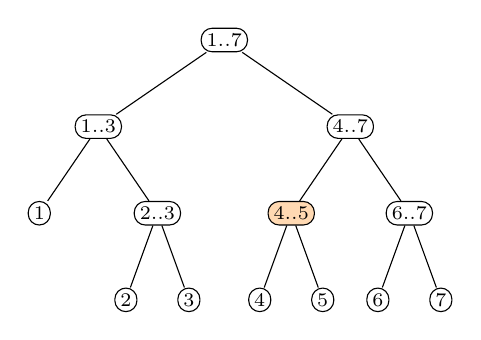
\begin{tikzpicture}[
  level distance=11mm,
  level 1/.style={sibling distance=32mm},
  level 2/.style={sibling distance=15mm},
  level 3/.style={sibling distance=8mm},
  every node/.style={draw,rounded corners,font=\scriptsize,inner sep=2pt,fill=white},
  edge from parent/.style={draw}]
\node {$1..7$}
  child { node {$1..3$}
    child { node {$1$} }
    child { node {$2..3$} child { node {$2$} } child { node {$3$} } } }
  child { node {$4..7$}
    child { node[fill=orange!30] {$4..5$} child { node {$4$} } child { node {$5$} } }
    child { node {$6..7$} child { node {$6$} } child { node {$7$} } } };
\end{tikzpicture}

\vspace{1mm}
\scriptsize Cluster tree of the balanced bisection of $1,\dots,7$.
\end{column}
\begin{column}{0.48\textwidth}
\centering
% T_3 in post-order (edges 1-3, 2-3, 4-6, 5-6, 3-7, 6-7) with the clusters boxed
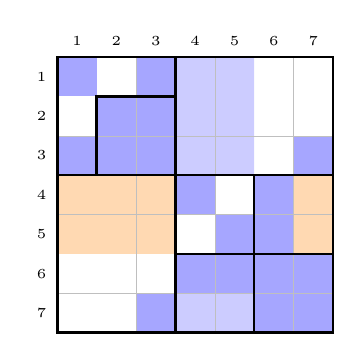
\begin{tikzpicture}[x=5mm,y=-5mm]
\fill[orange!30] (0,3) rectangle (3,5) (5,3) rectangle (7,5);
\fill[blue!20] (3,0) rectangle (5,3) (3,5) rectangle (5,7);
\foreach \i in {1,...,7} \fill[nz] (\i-1,\i-1) rectangle (\i,\i);
\foreach \c/\p in {1/3,2/3,4/6,5/6,3/7,6/7} {
  \fill[nz] (\c-1,\p-1) rectangle (\c,\p);
  \fill[nz] (\p-1,\c-1) rectangle (\p,\c);}
\draw[gray!50,line width=0.2pt] (0,0) grid (7,7);
\foreach \a/\b in {1/7,1/3,4/7,2/3,4/5,6/7} \draw[line width=0.9pt] (\a-1,\a-1) rectangle (\b,\b);
\foreach \k in {1,...,7} {\node[font=\tiny] at (\k-0.5,-0.4) {$\k$}; \node[font=\tiny] at (-0.4,\k-0.5) {$\k$};}
\end{tikzpicture}

\vspace{1mm}
\scriptsize $\mathrm{T}_3$ in post-order; boxes: clusters. For $\tau=\{4,5\}$:
\textcolor{orange!90!black}{$\mathrm{T}(\tau,\bar\tau)$}, \textcolor{blue!70!black}{$\mathrm{T}(\bar\tau,\tau)$}.
\end{column}
\end{columns}

\vspace{2mm}
\footnotesize
\begin{itemize}
\item \textbf{Ordering:} the nodes are numbered $1,\dots,K$ (here the post-order).
\item \textbf{Cluster tree:} a binary tree of index sets, the \emph{clusters} $\tau$. The root is $\{1,\dots,K\}$, every
  cluster is split into two consecutive intervals, and the leaves are single nodes.
\item \textbf{HSS} stores, for every cluster $\tau$ with complement $\bar\tau$, the off-diagonal blocks
  $\mathrm{T}(\tau,\bar\tau)$ and $\mathrm{T}(\bar\tau,\tau)$ in low-rank form, with bases nested along the tree.
  Its cost is governed by their ranks; both choices (ordering and cluster tree) are ours.
\end{itemize}
\end{frame}

\begin{frame}{The ranks depend on the ordering and the partition, not on $\mathrm{T}_k$ alone}
\begin{columns}[T]
\begin{column}{0.53\textwidth}
\footnotesize
Each format fixes \emph{which} sets $A$ appear as Hankel blocks:
\begin{itemize}
\item \textbf{SSS:} an ordering of the nodes; $A$ = every prefix of it.
\item \textbf{HSS:} an ordering and a cluster tree; $A$ = every cluster (an interval of the ordering).
\item \textbf{TQS:} a tree graph on the nodes; $A$ = one side of an edge. The ordering plays no role, the graph does.
\end{itemize}
Since $\operatorname{rank}\mathrm{T}^{-1}(\bar{A},A)=\operatorname{rank}\mathrm{T}(\bar{A},A)$, a rank belongs to the
pair (matrix, partition), not to the matrix.

\vspace{2mm}
\textbf{Same $\mathrm{T}_k^{-1}$, two TQS graphs:} on $\mathbb{G}_k$ all ranks are $1$; on the line graph
$1-2-\cdots-K$ in post-order (i.e.\ SSS) they reach $k-1$.

\vspace{2mm}
\alert{Rest of this section:} the paper's choices (post-order, balanced bisection; TQS on $\mathbb{G}_k$).
\end{column}
\begin{column}{0.45\textwidth}
\footnotesize
\textbf{Same $\mathrm{T}_k^{-1}$, two orderings} of the nodes (pictured on the next slide):

\vspace{1mm}
\raggedright
\scriptsize
\textbf{post-order} (used so far): left subtree, then right subtree, then the node; parents come after their
children, the root is last.\\
\textbf{level order} (breadth-first): root first, then each level from left to right.

\vspace{1mm}
\centering
\footnotesize
\renewcommand{\arraystretch}{1.0}
\begin{tabular}{rr|cc|cc}
\toprule
 & & \multicolumn{2}{c|}{SSS} & \multicolumn{2}{c}{HSS} \\
$k$ & $K$ & post & level & post & level \\
\midrule
4 & 15 & 3 & 4 & 3 & 4 \\
5 & 31 & 4 & 8 & 4 & 8 \\
6 & 63 & 5 & 16 & 4 & 16 \\
7 & 127 & 6 & 32 & 5 & 32 \\
8 & 255 & 7 & 64 & 7 & 64 \\
\bottomrule
\end{tabular}

\vspace{1mm}
\raggedright
\scriptsize
Largest Hankel-block rank, measured. In level order, the prefix ``all levels but the leaves'' has $2^{k-1}$
border edges from $2^{k-2}$ parents: rank $2^{k-2}=(K+1)/4$, no compression at all.
\end{column}
\end{columns}
\end{frame}

{\renewcommand{\treey}{5mm}\renewcommand{\spyunit}{1.9mm}
\begin{frame}{Post-order versus level order: the worst SSS cut of $\mathrm{T}_4$}
\begin{columns}[T]
\begin{column}{0.49\textwidth}
\centering
\textbf{post-order}\\
\treefour{1,2,3,4,5,6,7,8,9,10,11}{7/15,10/14,11/13}

\spyfour{\fill[hank] (0,11) rectangle (11,15); \fill[hank] (11,0) rectangle (15,11);}
        {15/7,14/10,13/11,7/15,10/14,11/13}

\vspace{1mm}
\raggedright
\scriptsize
Prefix $A=\{1,\dots,11\}$ = three complete subtrees. $3$ border edges with distinct end points:
rank $3$. In general at most $k-1$.
\end{column}
\begin{column}{0.49\textwidth}
\centering
\textbf{level order}\\
\treefourlevel{15,7,14,3,6,10,13}{1/3,2/3,4/6,5/6,8/10,9/10,11/13,12/13}

\spyfourwith{\levelfouredges}{\fill[hank] (0,7) rectangle (7,15); \fill[hank] (7,0) rectangle (15,7);}
        {8/4,9/4,10/5,11/5,12/6,13/6,14/7,15/7,4/8,4/9,5/10,5/11,6/12,6/13,7/14,7/15}

\vspace{1mm}
\raggedright
\scriptsize
Prefix $A=\{1,\dots,7\}$ = the top three levels. $8$ border edges, but only $4$ distinct parents:
rank $4$. In general $2^{k-2}=(K+1)/4$.
\end{column}
\end{columns}
\end{frame}
}

{\renewcommand{\treey}{6mm}\renewcommand{\spyunit}{2.5mm}
\begin{frame}{HSS, balanced bisection: one border edge per level near the root}
\label{sl:hssbisect}
\begin{columns}[T]
\begin{column}{0.48\textwidth}
\centering
\treefour{12,13,14,15}{11/13,10/14,7/15}

\vspace{1mm}
\spyfour{\fill[hank] (11,0) rectangle (15,11); \fill[hank] (0,11) rectangle (11,15);}
        {11/13,10/14,7/15,13/11,14/10,15/7}
\end{column}
\begin{column}{0.50\textwidth}
\footnotesize
HSS uses the balanced bisection of $1,\dots,K$ (as in the paper), e.g.\ for $k=4$:
\[
\{1..15\}\to\{1..7\},\{8..15\},
\]
\[
\{8..15\}\to\{8..11\},\{12..15\},\ \dots
\]
Cluster $A=\{12,\dots,15\}$ (orange):
\begin{itemize}
\item border edges $(13,11)$, $(14,10)$, $(15,7)$, so $\Ecount(A)=3$;
\item the shaded Hankel blocks of $\mathrm{T}_4$ hold three nonzeros (red) in distinct rows and columns;
\item hence $\operatorname{rank}\mathrm{T}_4^{-1}(\bar{A},A)=3$.
\end{itemize}

\vspace{1mm}
In general the clusters that contain the root also contain a piece of every level, and each piece is cut off from
its parent: HSS ranks grow like $k-1$.

Measured largest HSS rank: $3,4,4,5,7,8,8$ for $k=4,\dots,10$.
\end{column}
\end{columns}
\end{frame}
}

{\renewcommand{\treey}{6mm}\renewcommand{\spyunit}{2.5mm}
\begin{frame}{SSS: a post-order prefix is a union of up to $k-1$ subtrees}
\begin{columns}[T]
\begin{column}{0.48\textwidth}
\centering
\treefour{1,2,3,4,5,6,7,8,9,10,11}{7/15,10/14,11/13}

\vspace{1mm}
\spyfour{\fill[hank] (0,11) rectangle (11,15); \fill[hank] (11,0) rectangle (15,11);}
        {15/7,14/10,13/11,7/15,10/14,11/13}
\end{column}
\begin{column}{0.50\textwidth}
\footnotesize
SSS stores the Hankel blocks of the cuts $A=\{1,\dots,i\}$, $\bar{A}=\{i+1,\dots,K\}$.

\vspace{2mm}
In post-order, $\{1,\dots,i\}$ is a disjoint union of complete subtrees. Each one, except possibly a left/right
pair of siblings, contributes one border edge to its parent.

\vspace{2mm}
Cut $i=11$ in $\mathrm{T}_4$: subtrees rooted at $7$, $10$, $11$, border edges $(7,15)$, $(10,14)$, $(11,13)$,
rank $3$. (It is the complement of the HSS cluster on the previous slide.)

\vspace{2mm}
Measured on $\mathrm{T}_k^{-1}$: largest SSS rank $k-1$ and average about $k/2$, so the ranks are large at
\emph{most} cuts, not only at a few.
\end{column}
\end{columns}
\end{frame}
}

\begin{frame}{TQS on the adjacency graph: spinners of $\mathrm{T}_k$}
\footnotesize
Take $\mathbb{G}_k$ itself as the TQS graph, with rank profile $\rho_e=1$ for every edge.
Rows of $\mathrm{S}^i$: destination (edge to a neighbour, or the output); columns: source (edge from a neighbour, or the input).

\vspace{1mm}
\[
\mathrm{S}^K=
\begin{bNiceMatrix}[first-row,first-col]
 & \lc(K) & \rc(K) & \mathrm{Inp} \\
\lc(K) & 0 & 0 & p^K_{\lc(K)} \\
\rc(K) & 0 & 0 & p^K_{\rc(K)} \\
\mathrm{Out} & 1 & 1 & d^K
\end{bNiceMatrix},
\qquad
\mathrm{S}^i=
\begin{bNiceMatrix}[first-row,first-col]
 & \Par(i) & \mathrm{Inp} \\
\Par(i) & 0 & b^i_{\Par(i)} \\
\mathrm{Out} & 1 & d^i
\end{bNiceMatrix}\ (i \text{ leaf}),
\]
\[
\mathrm{S}^i=
\begin{bNiceMatrix}[first-row,first-col]
 & \lc(i) & \rc(i) & \Par(i) & \mathrm{Inp} \\
\lc(i) & 0 & 0 & 0 & p^i_{\lc(i)} \\
\rc(i) & 0 & 0 & 0 & p^i_{\rc(i)} \\
\Par(i) & 0 & 0 & 0 & b^i_{\Par(i)} \\
\mathrm{Out} & 1 & 1 & 1 & d^i
\end{bNiceMatrix}\ (i \text{ interior}).
\]
Edge-to-edge operators are $0$ (nothing travels more than one edge) and edge-to-output operators are $1$.
This representation is neither SSS nor HSS.
\end{frame}

\begin{frame}{TQS of the inverse: same graph, same rank profile}
\begin{columns}[T]
\begin{column}{0.44\textwidth}
\centering
\treefour{8,9,10,11,12,13,14}{14/15}

\vspace{2mm}
\scriptsize $A$ = subtree of $14$: one border edge, $(14,15)$.\\
Every edge of $\mathbb{G}_k$ splits $\mathbb{V}$ like this.
\end{column}
\begin{column}{0.54\textwidth}
\footnotesize
Every Hankel block a TQS representation on $\mathbb{G}_k$ needs is induced by a subtree $A$ hanging off one edge, so
$\operatorname{rank}\mathrm{T}_k^{-1}(\bar{A},A)\le\Ecount(A)=1$.

\vspace{1mm}
\textbf{TQS inverse proposition.} $\mathrm{T}_k^{-1}$ is TQS on $\mathbb{G}_k$ with the same rank profile,
$\rho_e=1$ for all $e$. The spinners keep their sizes, but the zeros fill in, e.g.\ for an interior node
\[
\mathrm{S}^i=
\begin{bNiceMatrix}[first-row,first-col]
 & \lc(i) & \rc(i) & \Par(i) & \mathrm{Inp} \\
\lc(i) & 0 & \mathrm{V}^i_{\lc,\rc} & \mathrm{W}^i_{\lc,\Par} & \mathrm{P}^i_{\lc(i)} \\
\rc(i) & \mathrm{V}^i_{\rc,\lc} & 0 & \mathrm{W}^i_{\rc,\Par} & \mathrm{P}^i_{\rc(i)} \\
\Par(i) & \mathrm{U}^i_{\Par,\lc} & \mathrm{U}^i_{\Par,\rc} & 0 & \mathrm{B}^i_{\Par(i)} \\
\mathrm{Out} & \mathrm{C}^i_{\lc(i)} & \mathrm{C}^i_{\rc(i)} & \mathrm{Q}^i_{\Par(i)} & \mathrm{D}^i
\end{bNiceMatrix},
\]
all scalars ($\lc,\rc,\Par$ short for $\lc(i),\rc(i),\Par(i)$).

\vspace{1mm}
Parameters: $2^{k-1}$ leaves ($2\times 2$), $2^{k-1}-2$ interior nodes ($4\times 4$), one root ($3\times 3$):
\[
4\cdot 2^{k-1}+16\,(2^{k-1}-2)+9=10K-13=\Theta(K).
\]
\end{column}
\end{columns}
\end{frame}

\begin{frame}{Storage of $\mathrm{T}_k^{-1}$: measured}
\footnotesize
Random $d^i,b^i_{\Par(i)},p^{\Par(i)}_i$; ranks computed numerically; parameters counted with dense generators
(\texttt{verify\_binary\_tree\_inverse.jl}). SSS, HSS: post-order, balanced bisection; TQS: on $\mathbb{G}_k$.
Other choices give other numbers.

\vspace{1mm}
\centering
\renewcommand{\arraystretch}{1.0}
\begin{tabular}{rr|ccc|rrr}
\toprule
 & & \multicolumn{3}{c|}{largest Hankel-block rank} & \multicolumn{3}{c}{parameters$/K$} \\
$k$ & $K$ & TQS on $\mathbb{G}_k$ & HSS & SSS & TQS & HSS & SSS \\
\midrule
4 & 15 & 1 & 3 & 3 & 9.1 & 12.2 & 13.3 \\
5 & 31 & 1 & 4 & 4 & 9.6 & 16.0 & 19.1 \\
6 & 63 & 1 & 4 & 5 & 9.8 & 19.2 & 25.9 \\
7 & 127 & 1 & 5 & 6 & 9.9 & 21.4 & 33.8 \\
8 & 255 & 1 & 7 & 7 & 9.9 & 23.0 & 42.7 \\
9 & 511 & 1 & 8 & 8 & 10.0 & 24.6 & 52.6 \\
10 & 1023 & 1 & 8 & 9 & 10.0 & 26.3 & 63.6 \\
\bottomrule
\end{tabular}


\raggedright
\begin{itemize}
\item TQS: $10K-13$ parameters, $\Theta(K)$; the sparse $\mathrm{T}_k$ itself has $3K-2$ nonzeros.
\item HSS (balanced bisection): parameters$/K$ grows by about $1.6$ per level, i.e.\ $\Theta(K\log K)$, as stated
  in the paper. A different cluster tree brings this down to $9K-10$ (next slides).
\item SSS: average rank $\approx k/2$, and the $r\times r$ transition matrices make parameters$/K$ grow
  quadratically in $k$, i.e.\ $\Theta(K\log^2 K)$ with dense generators.
  The paper quotes $\Theta(K\log K)$; that count holds for the sum of the SSS ranks.
\end{itemize}
\end{frame}

\section{The example of the original paper is misleading}

{\renewcommand{\spyunit}{1.65mm}
\begin{frame}{Can HSS do as well as TQS? Yes, with a subtree-aligned cluster tree}
\begin{columns}[T]
\begin{column}{0.27\textwidth}
\centering
\scriptsize\textbf{balanced bisection (paper)}\\[1mm]
\spyfourclusters{1/15,1/7,8/15,1/3,4/7,2/3,4/5,6/7,8/11,12/15,8/9,10/11,12/13,14/15}

\vspace{2mm}
\textbf{subtree-aligned}\\[1mm]
\spyfourclusters{1/15,1/7,8/15,8/14,1/3,4/7,4/6,2/3,5/6,8/10,11/14,11/13,9/10,12/13}
\end{column}
\begin{column}{0.71\textwidth}
\footnotesize
\textbf{Subtree-aligned cluster tree} (post-order, $\mathrm{T}_k$ unchanged). With
$\mathcal{R}(v):=\mathcal{S}(\rc(v))\cup\{v\}$, split
\[
\mathcal{S}(v)\;\to\;\mathcal{S}(\lc(v)),\ \mathcal{R}(v),\qquad
\mathcal{R}(v)\;\to\;\mathcal{S}(\rc(v)),\ \{v\},
\]
down to single nodes. Post-order lists $\mathcal{S}(v)$ as
$[\mathcal{S}(\lc(v)),\,\mathcal{S}(\rc(v)),\,v]$, so every cluster is an interval.

\vspace{1mm}
Left: boxes are the clusters of size $\geq 2$ for $\mathrm{T}_4$. The two trees agree at the top
($\{1..7\},\{8..15\}$) but split $\{8..15\}$ differently: $\{8..11\},\{12..15\}$ versus
$\{8..14\}=\mathcal{S}(14)$, $\{15\}$.

\vspace{2mm}
\textbf{Measured} on $\mathrm{T}_k^{-1}$, $k=2,\dots,9$: every HSS Hankel block has rank $1$, and the
representation has $9K-10$ parameters, slightly \emph{fewer} than TQS on $\mathbb{G}_k$ ($10K-13$).

\vspace{2mm}
\alert{So the $\log K$ gap of the paper comes from the balanced bisection, not from HSS itself.} HSS ranks only
depend on the cluster \emph{sets}; in-order ($\mathcal{S}(\lc(v)),v,\mathcal{S}(\rc(v))$) with the same sets
gives the same ranks.
\end{column}
\end{columns}
\end{frame}
}

\begin{frame}{The subtree-aligned cluster tree, drawn on $\mathbb{G}_4$}
\footnotesize
Each round splits every cluster in two:
$\textcolor{clS}{\mathcal{S}(v)}\to\textcolor{clS}{\mathcal{S}(\lc(v))},\ \textcolor{clR}{\mathcal{R}(v)}$ \ cuts the edge
$(\lc(v),v)$; \ $\textcolor{clR}{\mathcal{R}(v)}\to\textcolor{clS}{\mathcal{S}(\rc(v))},\ \textcolor{clV}{\{v\}}$ cuts
the edge $(\rc(v),v)$.

\vspace{2mm}
\centering
\begin{tabular}{ccc}
\clusterpanel{1,2,3,4,5,6,7}{8,9,10,11,12,13,14,15}{}
  {1/3,2/3,4/6,5/6,3/7,6/7}{8/10,9/10,11/13,12/13,10/14,13/14,14/15} &
\clusterpanel{1,2,3,8,9,10,11,12,13,14}{4,5,6,7}{15}
  {1/3,2/3,8/10,9/10,11/13,12/13,10/14,13/14}{4/6,5/6,6/7} &
\clusterpanel{1,4,5,6,8,9,10}{2,3,11,12,13,14}{7,15}
  {4/6,5/6,8/10,9/10}{2/3,11/13,12/13,13/14} \\[1mm]
\scriptsize round 1 & \scriptsize round 2 & \scriptsize round 3 \\
\scriptsize $\textcolor{clS}{\mathcal{S}(7)}$, $\textcolor{clR}{\mathcal{R}(15)}$ &
\scriptsize $\textcolor{clS}{\mathcal{S}(3)}$, $\textcolor{clR}{\mathcal{R}(7)}$, $\textcolor{clS}{\mathcal{S}(14)}$, $\textcolor{clV}{\{15\}}$ &
\scriptsize $\textcolor{clS}{\mathcal{S}(1)}$, $\textcolor{clR}{\mathcal{R}(3)}$, $\textcolor{clS}{\mathcal{S}(6)}$, $\textcolor{clV}{\{7\}}$,
  $\textcolor{clS}{\mathcal{S}(10)}$, $\textcolor{clR}{\mathcal{R}(14)}$
\end{tabular}

\vspace{2mm}
\raggedright
Blue $\textcolor{clS}{\mathcal{S}(v)}$: a whole subtree, one red edge leaves it. Orange
$\textcolor{clR}{\mathcal{R}(v)}=\mathcal{S}(\rc(v))\cup\{v\}$: two red edges leave it, \emph{both at its top node $v$}.
Grey: a single node, already a leaf of the cluster tree. This continues until every cluster is a single node
(at most $2k-2$ rounds). The balanced bisection instead cuts $\{8..15\}$ into $\{8..11\}$, $\{12..15\}$, which leaves
$\{12..15\}$ with three red edges at three different nodes (slide~\pageref{sl:hssbisect}).
\end{frame}

\begin{frame}{Theorem 1: subtree-aligned HSS is rank $1$ and linear}
\footnotesize
\begin{block}{Theorem 1}
For invertible $\mathrm{T}_k$ and the subtree-aligned cluster tree, every HSS Hankel block
$\mathrm{T}_k^{-1}(\bar{A},A)$ and $\mathrm{T}_k^{-1}(A,\bar{A})$, $A$ a cluster, has rank $\leq 1$. The HSS
representation with dense generators has $9K-10=\Theta(K)$ parameters.
\end{block}
\end{frame}

\section{A negative result}

\begin{frame}{Beyond $\mathrm{T}_k$, setting (1): TQS storage on a tree}
\label{sl:set1}
\begin{columns}[c]
\begin{column}{0.40\textwidth}
\centering
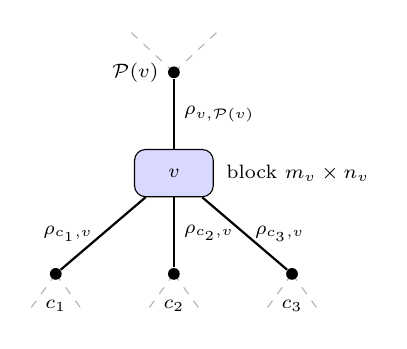
\begin{tikzpicture}[x=1cm,y=0.8cm,
  nd/.style={circle,fill,inner sep=1.5pt}, lab/.style={font=\scriptsize}]
\draw[gray!60,dashed] (0,1.6) -- (-0.6,2.3) (0,1.6) -- (0.6,2.3);
\foreach \x in {-1.5,0,1.5} \draw[gray!60,dashed] (\x,-1.6) -- (\x-0.35,-2.2) (\x,-1.6) -- (\x+0.35,-2.2);
\node[nd] (p) at (0,1.6) {};
\node[lab,left=2pt] at (p) {$\Par(v)$};
\foreach \k/\x in {1/-1.5,2/0,3/1.5} {\node[nd] (c\k) at (\x,-1.6) {}; \node[lab,below=6pt] at (c\k) {$c_\k$};}
\node[draw,rounded corners,fill=blue!15,minimum width=10mm,minimum height=6mm,font=\scriptsize] (v) at (0,0) {$v$};
\node[lab,right=1pt] at (v.east) {block $m_v\times n_v$};
\draw[thick] (v) -- (p) node[lab,midway,right] {$\rho_{v,\Par(v)}$};
\draw[thick] (v) -- (c1) node[lab,midway,left] {$\rho_{c_1,v}$};
\draw[thick] (v) -- (c2) node[lab,midway,right] {$\rho_{c_2,v}$};
\draw[thick] (v) -- (c3) node[lab,midway,right] {$\rho_{c_3,v}$};
\end{tikzpicture}

\vspace{2mm}
\scriptsize
total state dimension at $v$:\\
$D_v:=\sum_{e\ni v}\rho_e=\rho_{v,\Par(v)}+\rho_{c_1,v}+\rho_{c_2,v}+\rho_{c_3,v}$
\end{column}
\begin{column}{0.58\textwidth}
\centering
% spinner of v: edge widths 1 (parent), 2, 1, 1 (children); n_v = 2, m_v = 3
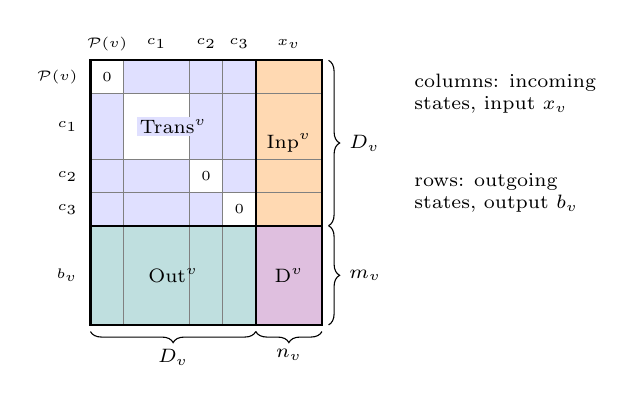
\begin{tikzpicture}[x=4.2mm,y=-4.2mm, lab/.style={font=\scriptsize}]
\fill[blue!12] (0,0) rectangle (5,5);
\foreach \a/\b in {0/1,1/3,3/4,4/5} \fill[white] (\a,\a) rectangle (\b,\b);
\fill[orange!30] (5,0) rectangle (7,5);
\fill[teal!25] (0,5) rectangle (5,8);
\fill[violet!25] (5,5) rectangle (7,8);
\foreach \t in {1,3,4,5} {\draw[gray] (\t,0) -- (\t,8); \draw[gray] (0,\t) -- (7,\t);}
\draw[thick] (0,0) rectangle (7,8);
\draw[thick] (5,0) -- (5,8) (0,5) -- (7,5);
\foreach \a/\b in {0/1,1/3,3/4,4/5} \node[font=\tiny] at ({(\a+\b)/2},{(\a+\b)/2}) {$0$};
\node[lab,fill=blue!12,inner sep=1pt] at (2.5,2.0) {$\mathrm{Trans}^v$};
\node[lab] at (6,2.5) {$\mathrm{Inp}^v$};
\node[lab] at (2.5,6.5) {$\mathrm{Out}^v$};
\node[lab] at (6,6.5) {$\mathrm{D}^v$};
\foreach \c/\l in {0.5/\Par(v),2/c_1,3.5/c_2,4.5/c_3,6/x_v} \node[font=\tiny,rotate=0] at (\c,-0.5) {$\l$};
\foreach \c/\l in {0.5/\Par(v),2/c_1,3.5/c_2,4.5/c_3,6.5/b_v} \node[font=\tiny,anchor=east] at (-0.1,\c) {$\l$};
\draw[decorate,decoration={brace,amplitude=4pt,mirror}] (0,8.2) -- (5,8.2) node[lab,midway,below=3pt] {$D_v$};
\draw[decorate,decoration={brace,amplitude=4pt,mirror}] (5,8.2) -- (7,8.2) node[lab,midway,below=3pt] {$n_v$};
\draw[decorate,decoration={brace,amplitude=4pt}] (7.2,0) -- (7.2,5) node[lab,midway,right=4pt] {$D_v$};
\draw[decorate,decoration={brace,amplitude=4pt}] (7.2,5) -- (7.2,8) node[lab,midway,right=4pt] {$m_v$};
\node[lab,align=left,anchor=west] at (9.5,1) {columns: incoming\\ states, input $x_v$};
\node[lab,align=left,anchor=west] at (9.5,4) {rows: outgoing\\ states, output $b_v$};
\end{tikzpicture}

\vspace{1mm}
\scriptsize Spinner $\mathrm{S}^v$ (here $\rho=1,2,1,1$, $n_v=2$, $m_v=3$).
\end{column}
\end{columns}

\vspace{3mm}
\footnotesize
$\mathrm{T}$ is TQS on a tree $\mathbb{G}=(\mathbb{V},\mathbb{E})$: node $v$ has a block of size $m_v\times n_v$, edge $e$
has state dimension $\rho_e$. The spinner of $v$ has
\[
\tau_v:=(D_v+m_v)(D_v+n_v)\ \text{entries},\qquad
\mathcal{T}_{\mathrm{TQS}}(\mathrm{T},\mathbb{G}):=\textstyle\sum_{v\in\mathbb{V}}\tau_v\quad\text{(TQS storage, dense spinners).}
\]
\end{frame}

\begin{frame}{Beyond $\mathrm{T}_k$, setting (2): HSS storage on a cluster tree}
\begin{columns}[c]
\begin{column}{0.50\textwidth}
\centering
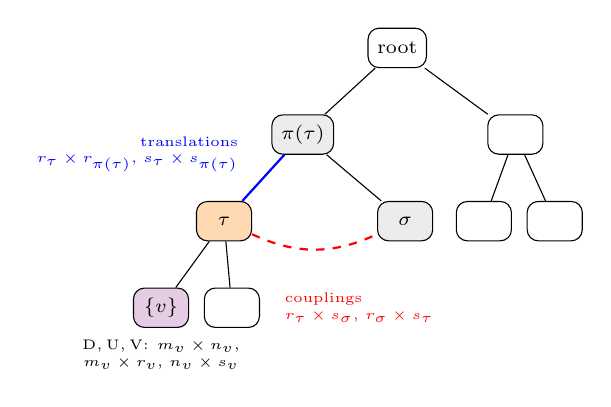
\begin{tikzpicture}[x=1cm,y=1cm,
  cl/.style={draw,rounded corners,minimum width=7mm,minimum height=5mm,font=\scriptsize,fill=white},
  lab/.style={font=\tiny}]
\node[cl] (root) at (0,0) {root};
\node[cl,fill=gray!15] (pi) at (-1.2,-1.1) {$\pi(\tau)$};
\node[cl] (o) at (1.5,-1.1) {};
\node[cl,fill=orange!30] (tau) at (-2.2,-2.2) {$\tau$};
\node[cl,fill=gray!15] (sig) at (0.1,-2.2) {$\sigma$};
\node[cl] (o2) at (1.1,-2.2) {};
\node[cl] (o3) at (2.0,-2.2) {};
\node[cl,fill=violet!20] (lv) at (-3.0,-3.3) {$\{v\}$};
\node[cl] (lw) at (-2.1,-3.3) {};
\draw (root) -- (pi) (root) -- (o) (pi) -- (sig) (o) -- (o2) (o) -- (o3) (tau) -- (lw) (tau) -- (lv);
\draw[thick,blue] (pi) -- (tau);
\node[lab,blue,align=right,anchor=east] at (-1.9,-1.35) {translations\\ $r_\tau\times r_{\pi(\tau)}$, $s_\tau\times s_{\pi(\tau)}$};
\draw[red,dashed,thick] (tau) to[bend right=25] (sig);
\node[lab,red,align=left,anchor=west] at (-1.55,-3.3) {couplings\\ $r_\tau\times s_\sigma$, $r_\sigma\times s_\tau$};
\node[lab,below=1pt,align=center] at (lv.south) {$\mathrm{D},\mathrm{U},\mathrm{V}$: $m_v\times n_v$,\\ $m_v\times r_v$, $n_v\times s_v$};
\end{tikzpicture}
\end{column}
\begin{column}{0.48\textwidth}
\centering
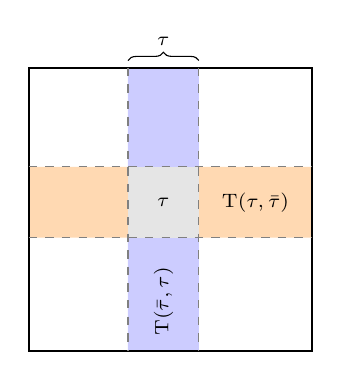
\begin{tikzpicture}[x=0.9mm,y=-0.9mm, lab/.style={font=\scriptsize}]
\fill[orange!30] (0,14) rectangle (14,24) (24,14) rectangle (40,24);
\fill[blue!20] (14,0) rectangle (24,14) (14,24) rectangle (24,40);
\fill[gray!20] (14,14) rectangle (24,24);
\draw[thick] (0,0) rectangle (40,40);
\draw[gray,dashed] (14,0) -- (14,40) (24,0) -- (24,40) (0,14) -- (40,14) (0,24) -- (40,24);
\node[lab] at (19,19) {$\tau$};
\node[lab,align=center] at (32,19) {$\mathrm{T}(\tau,\bar\tau)$};
\node[lab,align=center,rotate=90] at (19,33) {$\mathrm{T}(\bar\tau,\tau)$};
\draw[decorate,decoration={brace,amplitude=3pt}] (14,-1) -- (24,-1) node[lab,midway,above=2pt] {$\tau$};
\end{tikzpicture}

\vspace{1mm}
\scriptsize
Ordering of $\mathbb{V}$: every cluster $\tau$ is an interval.\\
\textcolor{orange!90!black}{row rank $r_\tau:=\operatorname{rank}\mathrm{T}(\tau,\bar\tau)$},
\textcolor{blue!70!black}{column rank $s_\tau:=\operatorname{rank}\mathrm{T}(\bar\tau,\tau)$}.
\end{column}
\end{columns}

\vspace{2mm}
\footnotesize
A binary cluster tree with leaves $\{v\}$; $\pi(\tau)$ is the parent and $\sigma$ the sibling of $\tau$. HSS stores
$\mathrm{T}$ through small generators attached to this tree (next slide).
\end{frame}

\begin{frame}{Beyond $\mathrm{T}_k$, setting (3): what HSS stores, and $\mathcal{T}_{\mathrm{HSS}}$}
\label{sl:set3}
\footnotesize
\textbf{One level of the cluster tree.} Let $\alpha,\beta$ be the two children of a cluster $\tau$. Then
\[
\mathrm{T}(\tau,\tau)=
\begin{bmatrix}
\mathrm{T}(\alpha,\alpha) & \mathrm{U}_\alpha\,\mathrm{B}_{\alpha\beta}\,\mathrm{V}_\beta^{\mathsf H}\\[2pt]
\mathrm{U}_\beta\,\mathrm{B}_{\beta\alpha}\,\mathrm{V}_\alpha^{\mathsf H} & \mathrm{T}(\beta,\beta)
\end{bmatrix},
\qquad
\mathrm{U}_\tau=\begin{bmatrix}\mathrm{U}_\alpha\mathrm{R}_\alpha\\ \mathrm{U}_\beta\mathrm{R}_\beta\end{bmatrix},\quad
\mathrm{V}_\tau=\begin{bmatrix}\mathrm{V}_\alpha\mathrm{R}'_\alpha\\ \mathrm{V}_\beta\mathrm{R}'_\beta\end{bmatrix}.
\]
$\mathrm{U}_\tau$ (columns $r_\tau$) spans the columns of $\mathrm{T}(\tau,\bar\tau)$, $\mathrm{V}_\tau$ (columns $s_\tau$)
spans the rows of $\mathrm{T}(\bar\tau,\tau)$; $(\cdot)^{\mathsf H}$ is the conjugate transpose. Only the leaves store
bases explicitly; a parent's bases are built from its children's (\emph{nested bases}).

\vspace{1mm}
\centering
\scriptsize
\renewcommand{\arraystretch}{1.1}
\begin{tabular}{@{}llll@{}}
\toprule
generator & stored for & role & size \\
\midrule
$\mathrm{D}_v$ & every leaf $\{v\}$ & diagonal block $\mathrm{T}(v,v)$ & $m_v\times n_v$ \\
$\mathrm{U}_v$, $\mathrm{V}_v$ & every leaf $\{v\}$ & row / column basis, stored explicitly & $m_v\times r_v$, \ $n_v\times s_v$ \\
$\mathrm{R}_\tau$, $\mathrm{R}'_\tau$ & every cluster $\tau\neq$ root & translation to parent's bases &
  $r_\tau\times r_{\pi(\tau)}$, \ $s_\tau\times s_{\pi(\tau)}$ \\
$\mathrm{B}_{\tau\sigma}$, $\mathrm{B}_{\sigma\tau}$ & every sibling pair $\tau,\sigma$ & coupling: block
  $\mathrm{T}(\tau,\sigma)$ & $r_\tau\times s_\sigma$, \ $r_\sigma\times s_\tau$ \\
\midrule
\textcolor{gray}{$\mathrm{U}_\tau$, $\mathrm{V}_\tau$} & \textcolor{gray}{$\tau$ not a leaf} &
  \textcolor{gray}{\emph{not stored}: built from children via $\mathrm{R}$, $\mathrm{R}'$} & \textcolor{gray}{---} \\
\bottomrule
\end{tabular}

\vspace{1mm}
\raggedright
\footnotesize
$\mathcal{T}_{\mathrm{HSS}}$ is the number of stored entries, i.e.\ the sum of the sizes in the table:
\[
\mathcal{T}_{\mathrm{HSS}}:=\underbrace{\textstyle\sum_{v}(m_vn_v+m_vr_v+n_vs_v)}_{\mathrm{D}_v,\ \mathrm{U}_v,\ \mathrm{V}_v}
+\underbrace{\textstyle\sum_{\tau\neq\text{root}}(r_\tau r_{\pi(\tau)}+s_\tau s_{\pi(\tau)})}_{\mathrm{R}_\tau,\ \mathrm{R}'_\tau}
+\underbrace{\textstyle\sum_{\text{siblings }\tau,\sigma}(r_\tau s_\sigma+r_\sigma s_\tau)}_{\mathrm{B}_{\tau\sigma},\ \mathrm{B}_{\sigma\tau}}.
\]
\end{frame}

\begin{frame}{Theorem 2: HSS emulates TQS on any tree}
\label{sl:thm2}\hypertarget{sl:thm2}{}
\footnotesize
\begin{block}{Theorem 2}
For every TQS matrix $\mathrm{T}$ on a tree $\mathbb{G}$ (any degrees, rank profile, block sizes) there is an ordering
and an HSS cluster tree with
\[
\mathcal{T}_{\mathrm{HSS}}\;\leq\;16\,\mathcal{T}_{\mathrm{TQS}}(\mathrm{T},\mathbb{G}).
\]
\end{block}

\end{frame}

\begin{frame}{How the cluster tree of Theorem 2 is built}
\footnotesize
Root the tree. Only two kinds of cluster occur:
\begin{itemize}
\item a \textbf{subtree} $\mathcal{S}(v)$: $v$ and all its descendants;
\item a \textbf{group} of sibling subtrees $\mathcal{S}(c_1)\cup\dots\cup\mathcal{S}(c_j)$, with
  $c_1,\dots,c_j\in\mathcal{C}(v)$ children of the same node $v$. The largest group is
  $C_v:=\bigcup_{c\in\mathcal{C}(v)}\mathcal{S}(c)=\mathcal{S}(v)\setminus\{v\}$, all descendants of $v$.
\end{itemize}

\vspace{1mm}
\textbf{Rules}, applied recursively from $\mathcal{S}(\text{root})=\mathbb{V}$:

\vspace{1mm}
\renewcommand{\arraystretch}{1.25}
\begin{tabular}{@{}lll@{}}
\toprule
& cluster & split \\
\midrule
1. & $\mathcal{S}(v)$, $v$ a leaf & it is $\{v\}$: a leaf of the cluster tree \\
2. & $\mathcal{S}(v)$, $v$ not a leaf & peel off the top node: $\mathcal{S}(v)\to\{v\},\ C_v$ \\
3. & group of $\geq2$ subtrees & two smaller groups of siblings, balanced by weight $\sum\rho_{c,v}$ \\
4. & group of one subtree $\mathcal{S}(c)$ & it is a subtree: apply rule 1 or 2 to $c$ \\
\bottomrule
\end{tabular}

\vspace{2mm}
\textbf{Why.} Every cluster has all its border edges at \emph{one} node: $\mathcal{S}(v)$ only the edge to
$\Par(v)$; a group of children of $v$ only edges to $v$; $\{v\}$ is a single node. So every HSS rank is bounded by
the state dimensions around one node. Balancing in rule 3 splits $d$ children in about $\log_2 d$ levels instead of
$d$, which keeps high-degree nodes at cost $O(d^2)$.
\end{frame}

\begin{frame}{The cluster tree of Theorem 2 on an example}
\begin{columns}[T]
\begin{column}{0.27\textwidth}
\centering
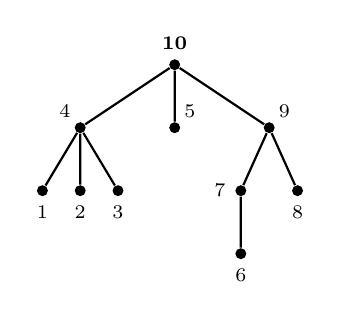
\begin{tikzpicture}[x=6mm,y=8mm, nd/.style={circle,fill,inner sep=1.4pt}, lab/.style={font=\scriptsize}]
\foreach \k/\x/\y in {10/0/0,4/-2/-1,5/0/-1,9/2/-1,1/-2.8/-2,2/-2/-2,3/-1.2/-2,7/1.4/-2,8/2.6/-2,6/1.4/-3}
  \node[nd] (n\k) at (\x,\y) {};
\draw[thick] (n10) -- (n4) (n10) -- (n5) (n10) -- (n9) (n4) -- (n1) (n4) -- (n2) (n4) -- (n3)
  (n9) -- (n7) (n9) -- (n8) (n7) -- (n6);
\node[lab,above=2pt] at (n10) {$\mathbf{10}$};
\node[lab,above left=0pt] at (n4) {$4$};
\node[lab,above right=0pt] at (n9) {$9$};
\node[lab,above right=0pt] at (n5) {$5$};
\foreach \k in {1,2,3,8,6} \node[lab,below=2pt] at (n\k) {$\k$};
\node[lab,left=2pt] at (n7) {$7$};
\end{tikzpicture}

\vspace{1mm}
\scriptsize
$K=10$, root $10$, post-order labels, $\rho_e=1$.

\vspace{1mm}
\setlength{\tabcolsep}{2pt}
\begin{tabular}{@{}ll@{}}
\tikz\fill[white,draw=black] (0,0) rectangle (2mm,2mm); & subtree $\mathcal{S}(v)$ \\
\tikz\fill[blue!15,draw=black] (0,0) rectangle (2mm,2mm); & $C_v$: all descendants of $v$ \\
\tikz\fill[orange!35,draw=black] (0,0) rectangle (2mm,2mm); & group of child subtrees \\
\tikz\fill[violet!20,draw=black] (0,0) rectangle (2mm,2mm); & single node
\end{tabular}
\end{column}
\begin{column}{0.72\textwidth}
\centering
% x = mean position of the leaves below, y = depth in the cluster tree
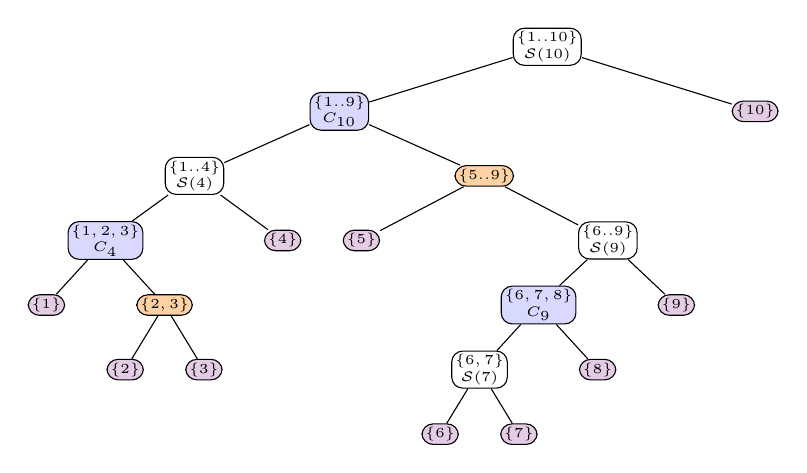
\begin{tikzpicture}[x=10mm,y=-8.2mm,
  cl/.style={draw,rounded corners,font=\tiny,inner sep=1.2pt,align=center},
  sv/.style={cl,fill=white}, cv/.style={cl,fill=blue!15}, gr/.style={cl,fill=orange!35},
  lf/.style={cl,fill=violet!20}]
\node[sv] (A) at (7.36,0) {$\{1..10\}$\\$\mathcal{S}(10)$};
\node[cv] (B) at (4.72,1) {$\{1..9\}$\\$C_{10}$};
\node[lf] (L10) at (10,1) {$\{10\}$};
\node[sv] (C) at (2.88,2) {$\{1..4\}$\\$\mathcal{S}(4)$};
\node[gr] (D) at (6.56,2) {$\{5..9\}$};
\node[cv] (E) at (1.75,3) {$\{1,2,3\}$\\$C_4$};
\node[lf] (L4) at (4,3) {$\{4\}$};
\node[lf] (L5) at (5,3) {$\{5\}$};
\node[sv] (F) at (8.13,3) {$\{6..9\}$\\$\mathcal{S}(9)$};
\node[lf] (L1) at (1,4) {$\{1\}$};
\node[gr] (G) at (2.5,4) {$\{2,3\}$};
\node[cv] (H) at (7.25,4) {$\{6,7,8\}$\\$C_9$};
\node[lf] (L9) at (9,4) {$\{9\}$};
\node[lf] (L2) at (2,5) {$\{2\}$};
\node[lf] (L3) at (3,5) {$\{3\}$};
\node[sv] (I) at (6.5,5) {$\{6,7\}$\\$\mathcal{S}(7)$};
\node[lf] (L8) at (8,5) {$\{8\}$};
\node[lf] (L6) at (6,6) {$\{6\}$};
\node[lf] (L7) at (7,6) {$\{7\}$};
\foreach \p/\c in {A/B,A/L10,B/C,B/D,C/E,C/L4,D/L5,D/F,E/L1,E/G,G/L2,G/L3,F/H,F/L9,H/I,H/L8,I/L6,I/L7}
  \draw (\p) -- (\c);
\end{tikzpicture}
\end{column}
\end{columns}

\vspace{1mm}
\footnotesize
Built with the rules of the previous slide. The two children of every cluster are disjoint and cover it; in
post-order every cluster is an interval.
\end{frame}

\begin{frame}{Proof of Theorem 2 (1): every rank is local to one node}
\footnotesize
\textbf{Strategy.} Charge every cluster of the cluster tree to one node $v$, its \emph{owner}, and show that the total
HSS storage charged to $v$ is $\leq 16\,\tau_v$, the size of the spinner of $v$. Summing over $v$ gives the theorem.

\vspace{1mm}
\begin{columns}[T]
\begin{column}{0.46\textwidth}
\centering
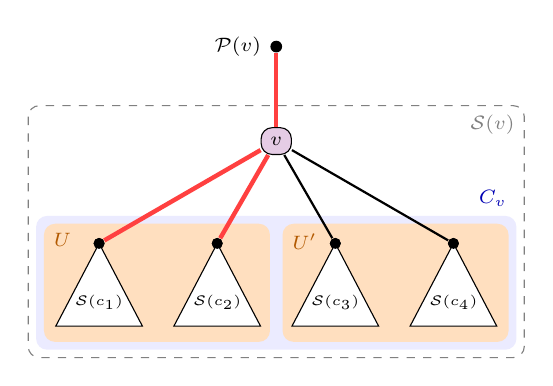
\begin{tikzpicture}[x=1cm,y=1cm, lab/.style={font=\scriptsize}]
% clusters (drawn first)
\draw[gray,dashed,rounded corners] (-3.15,0.45) rectangle (3.15,-2.75);
\node[lab,gray,anchor=north east] at (3.15,0.45) {$\mathcal{S}(v)$};
\fill[blue!8,rounded corners] (-3.05,-0.95) rectangle (3.05,-2.65);
\node[lab,blue!70!black,anchor=south east] at (3.05,-0.95) {$C_v$};
\fill[orange!25,rounded corners] (-2.95,-1.05) rectangle (-0.08,-2.55);
\fill[orange!25,rounded corners] (0.08,-1.05) rectangle (2.95,-2.55);
\node[lab,orange!70!black,anchor=north west] at (-2.95,-1.05) {$U$};
\node[lab,orange!70!black,anchor=north west] at (0.08,-1.05) {$U'$};
% tree
\node[circle,fill,inner sep=1.5pt] (p) at (0,1.2) {};
\node[lab,left=2pt] at (p) {$\Par(v)$};
\node[draw,rounded corners,fill=violet!20,font=\scriptsize] (v) at (0,0) {$v$};
\draw[hit,line width=1.6pt] (v) -- (p);
\foreach \k/\x in {1/-2.25,2/-0.75,3/0.75,4/2.25} {
  \node[circle,fill,inner sep=1.4pt] (c\k) at (\x,-1.3) {};
  \draw[fill=white] (\x,-1.3) -- (\x-0.55,-2.35) -- (\x+0.55,-2.35) -- cycle;
  \node[circle,fill,inner sep=1.4pt] at (\x,-1.3) {};
  \node[font=\tiny] at (\x,-2.05) {$\mathcal{S}(c_\k)$};}
\draw[hit,line width=1.6pt] (v) -- (c1) (v) -- (c2);
\draw[thick] (v) -- (c3) (v) -- (c4);
\end{tikzpicture}

\vspace{1mm}
\scriptsize
Red: border edges of $\mathcal{S}(v)$ (one) and of the group $U$ (all at $v$).
\end{column}
\begin{column}{0.52\textwidth}
\scriptsize
Rules 2 and 3 create exactly three kinds of cluster at a node $v$:

\vspace{1mm}
\renewcommand{\arraystretch}{1.25}
\setlength{\tabcolsep}{3pt}
\begin{tabular}{@{}lll@{}}
\toprule
cluster, owner $v$ & border edges & rank $\leq$ \\
\midrule
$\mathcal{S}(v)$ & $(v,\Par(v))$ & $\rho_{v,\Par(v)}\leq D_v$ \\
group $U\subseteq\mathcal{C}(v)$ & $(c,v)$, $c\in U$ & $w(U):=\sum_{c\in U}\rho_{c,v}\leq D_v$ \\
$\{v\}$ & all edges at $v$ & \begin{tabular}[t]{@{}l@{}}$r_v\leq\min(m_v,D_v)$,\\ $s_v\leq\min(n_v,D_v)$\end{tabular} \\
\bottomrule
\end{tabular}

\vspace{2mm}
\textbf{Why these bounds.} Every path from $\tau$ to $\bar\tau$ in the tree leaves $\tau$ through a border edge, so
$\mathrm{T}(\bar\tau,\tau)$ factors through the states on the border edges (GIRS):
\[
\operatorname{rank}\mathrm{T}(\bar\tau,\tau),\ \operatorname{rank}\mathrm{T}(\tau,\bar\tau)\;\leq\;\textstyle\sum_{e\text{ border}}\rho_e .
\]
All border edges of a cluster meet its owner $v$, so its ranks are bounded by $D_v$, a quantity of $v$ alone.
\end{column}
\end{columns}
\end{frame}

\begin{frame}{Proof of Theorem 2 (2): from products of ranks to squared ranks}
\begin{columns}[c]
\begin{column}{0.44\textwidth}
\centering
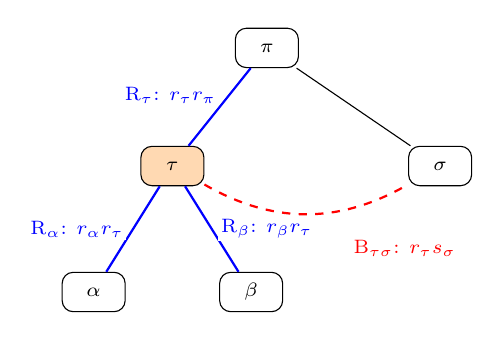
\begin{tikzpicture}[x=1cm,y=1cm,
  cl/.style={draw,rounded corners,minimum width=8mm,minimum height=5mm,font=\scriptsize,fill=white},
  lab/.style={font=\scriptsize}]
\node[cl] (pi) at (0,0) {$\pi$};
\node[cl,fill=orange!30] (tau) at (-1.2,-1.5) {$\tau$};
\node[cl] (sig) at (2.2,-1.5) {$\sigma$};
\node[cl] (al) at (-2.2,-3.1) {$\alpha$};
\node[cl] (be) at (-0.2,-3.1) {$\beta$};
\draw[thick,blue] (pi) -- (tau) node[lab,midway,above left=0pt,fill=white,inner sep=1pt] {$\mathrm{R}_\tau$: $r_\tau r_\pi$};
\draw (pi) -- (sig);
\draw[thick,blue] (tau) -- (al) node[lab,midway,left=2pt,fill=white,inner sep=1pt] {$\mathrm{R}_\alpha$: $r_\alpha r_\tau$};
\draw[thick,blue] (tau) -- (be) node[lab,midway,right=2pt,fill=white,inner sep=1pt] {$\mathrm{R}_\beta$: $r_\beta r_\tau$};
\draw[red,dashed,thick] (tau) to[bend right=30] (sig);
\node[lab,red,fill=white,inner sep=1pt] at (1.75,-2.55) {$\mathrm{B}_{\tau\sigma}$: $r_\tau s_\sigma$};
\end{tikzpicture}

\vspace{2mm}
\scriptsize
Cluster $\tau$ with parent $\pi$, sibling $\sigma$ and children $\alpha,\beta$: the four generators whose size contains
$r_\tau$.
\end{column}
\begin{column}{0.54\textwidth}
\footnotesize
Apart from the leaf terms, every term of $\mathcal{T}_{\mathrm{HSS}}$ is a product $xy$ of two ranks. Bound each by
$xy\leq\frac12x^2+\frac12y^2$: each product hands \emph{half a square} to each of its two factors.

\vspace{1mm}
\textbf{Count the halves that $r_\tau^2$ receives.} $r_\tau$ occurs in exactly four products:
\begin{itemize}
\item $r_\tau r_\pi$: translation $\mathrm{R}_\tau$ ($\tau$ as a \emph{child});
\item $r_\alpha r_\tau$, $r_\beta r_\tau$: translations $\mathrm{R}_\alpha,\mathrm{R}_\beta$ ($\tau$ as a \emph{parent});
\item $r_\tau s_\sigma$: coupling $\mathrm{B}_{\tau\sigma}$ with its \emph{sibling}.
\end{itemize}
So $r_\tau^2$ collects $4\times\frac12=2$. Likewise $s_\tau$ occurs in $\mathrm{R}'_\tau,\mathrm{R}'_\alpha,
\mathrm{R}'_\beta,\mathrm{B}_{\sigma\tau}$. (The root and the leaves occur in fewer products.) Hence
\[
\text{translations}+\text{couplings}\;\leq\;2\textstyle\sum_\tau\big(r_\tau^2+s_\tau^2\big),
\]
\[
\mathcal{T}_{\mathrm{HSS}}\leq\textstyle\sum_v\big(m_vn_v+m_vr_v+n_vs_v\big)+2\sum_\tau\big(r_\tau^2+s_\tau^2\big).
\]
\end{column}
\end{columns}
\end{frame}

\begin{frame}{Proof of Theorem 2 (3): balancing keeps the squared ranks small}
\begin{columns}[T]
\begin{column}{0.44\textwidth}
\footnotesize
\textbf{The danger: many groups at one node.} A node $v$ with $d$ children owns $d-1$ groups of child subtrees.
By part (1) a group $U$ has ranks $\leq w(U)$, so by part (2) it costs about $w(U)^2$.

\vspace{2mm}
The sum $\sum_U w(U)^2$ over the groups at $v$ must stay $O(d^2)$, the size of the spinner of $v$, and not grow to
$O(d^3)$.

\vspace{2mm}
How the children are grouped decides which (right).
\end{column}
\begin{column}{0.54\textwidth}
\centering
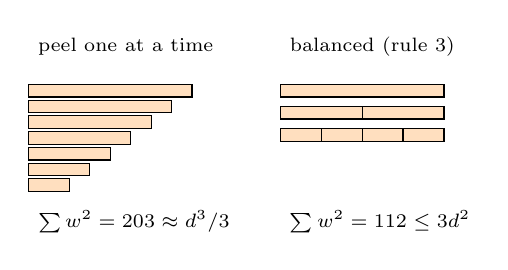
\begin{tikzpicture}[x=2.6mm,y=-2.0mm, lab/.style={font=\scriptsize}]
% peeling one child at a time, d = 8
\node[lab,anchor=west] at (0,-1.4) {peel one at a time};
\foreach \w [count=\i] in {8,7,6,5,4,3,2} \draw[fill=orange!25] (0,\i) rectangle (\w,\i+0.8);
\node[lab,anchor=north west] at (0,8.4) {$\sum w^2=203\approx d^3/3$};
% balanced halving, d = 8
\begin{scope}[xshift=32mm]
\node[lab,anchor=west] at (0,-1.4) {balanced (rule 3)};
\draw[fill=orange!25] (0,1) rectangle (8,1.8);
\foreach \a in {0,4} \draw[fill=orange!25] (\a,2.4) rectangle (\a+4,3.2);
\foreach \a in {0,2,4,6} \draw[fill=orange!25] (\a,3.8) rectangle (\a+2,4.6);
\node[lab,anchor=north west] at (0,8.4) {$\sum w^2=112\leq 3d^2$};
\end{scope}
\end{tikzpicture}

\vspace{1mm}
\scriptsize
Groups at a node with $d=8$ children of weight $1$ (bar length $=w(U)$).

\vspace{1mm}
\raggedright
\scriptsize
\textbf{Lemma.} With rule 3, every group with $\geq2$ subtrees splits into parts of weight $\leq\frac23$ of its own
(a heavy child, $\geq\frac13$, goes alone). Groups at depth $\ell$ below $C_v$ are disjoint and weigh
$\leq(\frac23)^\ell W_v$, with $W_v:=w(C_v)\leq D_v$. Hence
\[
\textstyle\sum_U w(U)^2\leq\sum_{\ell\geq0}(\frac23)^\ell W_v\cdot W_v=3W_v^2\leq 3D_v^2 .
\]
\end{column}
\end{columns}
\end{frame}

\begin{frame}{Proof of Theorem 2 (4): the charge at $v$ fits in the spinner of $v$}
\begin{columns}[c]
\begin{column}{0.38\textwidth}
\centering
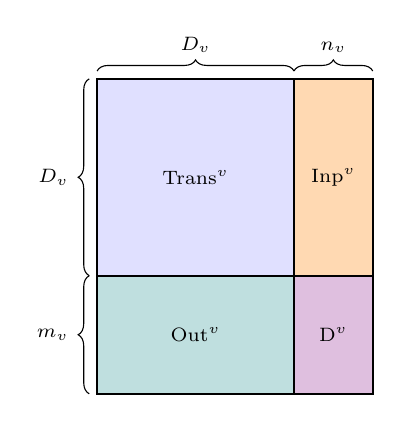
\begin{tikzpicture}[x=5mm,y=-5mm, lab/.style={font=\scriptsize}]
\fill[blue!12] (0,0) rectangle (5,5);
\fill[orange!30] (5,0) rectangle (7,5);
\fill[teal!25] (0,5) rectangle (5,8);
\fill[violet!25] (5,5) rectangle (7,8);
\draw[thick] (0,0) rectangle (7,8);
\draw[thick] (5,0) -- (5,8) (0,5) -- (7,5);
\node[lab] at (2.5,2.5) {$\mathrm{Trans}^v$};
\node[lab] at (6,2.5) {$\mathrm{Inp}^v$};
\node[lab] at (2.5,6.5) {$\mathrm{Out}^v$};
\node[lab] at (6,6.5) {$\mathrm{D}^v$};
\draw[decorate,decoration={brace,amplitude=4pt}] (0,-0.2) -- (5,-0.2) node[lab,midway,above=3pt] {$D_v$};
\draw[decorate,decoration={brace,amplitude=4pt}] (5,-0.2) -- (7,-0.2) node[lab,midway,above=3pt] {$n_v$};
\draw[decorate,decoration={brace,amplitude=4pt,mirror}] (-0.2,0) -- (-0.2,5) node[lab,midway,left=4pt] {$D_v$};
\draw[decorate,decoration={brace,amplitude=4pt,mirror}] (-0.2,5) -- (-0.2,8) node[lab,midway,left=4pt] {$m_v$};
\end{tikzpicture}

\vspace{1mm}
\scriptsize
Spinner of $v$: $\tau_v=\underbrace{D_v^2}_{\mathrm{Trans}}+\underbrace{(m_v+n_v)D_v}_{\mathrm{Inp},\,\mathrm{Out}}
+\underbrace{m_vn_v}_{\mathrm{D}}$ entries.
\end{column}
\begin{column}{0.61\textwidth}
\footnotesize
HSS storage charged to $v$ (factor $2$ from part (2), group sum from part (3)):

\vspace{1mm}
\scriptsize
\renewcommand{\arraystretch}{1.3}
\setlength{\tabcolsep}{2pt}
\begin{tabular}{@{}lll@{}}
\toprule
clusters owned by $v$ & charge & spinner \\
\midrule
$\mathcal{S}(v)$: $r^2+s^2\leq 2D_v^2$ & $2\cdot2D_v^2$ & \multirow{2}{*}{\tikz\fill[blue!12,draw=black] (0,0) rectangle (2mm,2mm); $16\,D_v^2$} \\
groups $U$: $\sum(r^2+s^2)\leq2\cdot3D_v^2$ & $2\cdot6D_v^2$ & \\
$\{v\}$: $r_v^2+s_v^2\leq(m_v+n_v)D_v$ & $2(m_v+n_v)D_v$ & \multirow{2}{*}{\tikz\fill[orange!30,draw=black] (0,0) rectangle (2mm,2mm); $3(m_v+n_v)D_v$} \\
$\{v\}$: bases $\mathrm{U}_v,\mathrm{V}_v$ & $(m_v+n_v)D_v$ & \\
$\{v\}$: $\mathrm{D}_v$ & $m_vn_v$ & \tikz\fill[violet!25,draw=black] (0,0) rectangle (2mm,2mm); $m_vn_v$ \\
\bottomrule
\end{tabular}

\vspace{2mm}
\footnotesize
Each region of the spinner pays for at most $16$ times its own size:
\[
\text{charge}(v)\;\leq\;16D_v^2+3(m_v+n_v)D_v+m_vn_v\;\leq\;16\,\tau_v .
\]
Every cluster has exactly one owner, so summing over $v$:
\[
\mathcal{T}_{\mathrm{HSS}}\;\leq\;16\textstyle\sum_v\tau_v=16\,\mathcal{T}_{\mathrm{TQS}}(\mathrm{T},\mathbb{G}).\qquad\square
\]
\end{column}
\end{columns}
\end{frame}

\begin{frame}{Corollary: TQS on a tree is never asymptotically more compact than HSS}
\label{sl:cor3}\hypertarget{sl:cor3}{}
\footnotesize
For a matrix $\mathrm{T}$ define the optimal storage of each format:
\[
\mathcal{T}^{*}_{\mathrm{HSS}}(\mathrm{T}):=\min_{\substack{\text{orderings,}\\\text{cluster trees}}}\mathcal{T}_{\mathrm{HSS}},
\qquad
\mathcal{T}^{*}_{\mathrm{TQS}}(\mathrm{T}):=\min_{\substack{\text{trees }\mathbb{G},\ \text{TQS}\\\text{representations of }\mathrm{T}\text{ on }\mathbb{G}}}
\mathcal{T}_{\mathrm{TQS}}(\mathrm{T},\mathbb{G}),
\]
with $\mathcal{T}_{\mathrm{HSS}}$ and $\mathcal{T}_{\mathrm{TQS}}$ as on slides~\pageref{sl:set1} and~\pageref{sl:set3} (exact ranks, dense
generators).

\vspace{2mm}
\begin{block}{Corollary 3}
For every matrix $\mathrm{T}$,
\[
\mathcal{T}^{*}_{\mathrm{HSS}}(\mathrm{T})\;\leq\;16\,\mathcal{T}^{*}_{\mathrm{TQS}}(\mathrm{T}).
\]
Consequently, for every family of matrices $(\mathrm{T}_K)_{K\geq1}$,
\[
\mathcal{T}^{*}_{\mathrm{HSS}}(\mathrm{T}_K)=O\big(\mathcal{T}^{*}_{\mathrm{TQS}}(\mathrm{T}_K)\big),
\qquad\text{i.e.}\qquad
\mathcal{T}^{*}_{\mathrm{TQS}}(\mathrm{T}_K)=o\big(\mathcal{T}^{*}_{\mathrm{HSS}}(\mathrm{T}_K)\big)\ \text{is impossible.}
\]
\end{block}

\textit{Proof.} Take a tree $\mathbb{G}$ and a TQS representation of $\mathrm{T}$ on $\mathbb{G}$ attaining
$\mathcal{T}^{*}_{\mathrm{TQS}}(\mathrm{T})$. Theorem 2 gives an ordering and a cluster tree with
$\mathcal{T}_{\mathrm{HSS}}\leq16\,\mathcal{T}_{\mathrm{TQS}}(\mathrm{T},\mathbb{G})=16\,\mathcal{T}^{*}_{\mathrm{TQS}}(\mathrm{T})$,
and $\mathcal{T}^{*}_{\mathrm{HSS}}(\mathrm{T})$ is at most that. \hfill$\square$

\vspace{2mm}
In words: an advantage of TQS over HSS in storage, as for $\mathrm{T}_k^{-1}$ with the balanced bisection, can only
come from the choice of ordering and cluster tree, never from the format itself.
\end{frame}

\begin{frame}{Measured on random trees}
\footnotesize
Scalar nodes, random entries, parameters$/K$ with dense generators
(\texttt{verify\_hss\_emulates\_tqs.jl}). Trees: random recursive (each new node attached to a random earlier one);
a path of $\approx\sqrt{K}$ hubs with the other nodes attached to random hubs; a star.

\vspace{2mm}
\centering
\textbf{TQS matrices} ($\rho_e=1$), Theorem 2\\[1mm]
\begin{tabular}{lr|r|rr}
\toprule
tree & $K$ & TQS & HSS, Thm 2 & HSS, bisection \\
\midrule
random & 100 & 10.9 & 14.8 & 36.4 \\
random & 400 & 10.9 & 14.4 & 45.2 \\
hubs & 100 & 17.8 & 33.7 & 55.3 \\
hubs & 400 & 28.4 & 64.8 & 118.9 \\
star & 100 & 104.0 & 294.9 & 298.8 \\
star & 400 & 404.0 & 1194.8 & 1198.8 \\
\bottomrule
\end{tabular}

\vspace{1mm}
HSS$/$TQS $\leq 3$ throughout, well below $16$.

\vspace{3mm}
\raggedright
\textbf{Caveats.} Exact ranks (no compression tolerance); storage with dense generators; the cluster trees can be
$\Theta(K)$ deep (e.g.\ on a path), so nothing is claimed about solver depth or about HSS restricted to balanced
cluster trees.
\end{frame}

\section{Conclusions}

\begin{frame}{Can the TQS format give asymptotically more compression than pure HSS?}
\label{sl:answer}\hypertarget{sl:answer}{}
\vfill
\centering
{\Huge\bfseries No.}
\vfill
\end{frame}

\end{document}
